\begin{song}{Härjarvisan}
	
%	\original{Gärdebylåten}\\
%	\songtext{Text: Hasse Alfredsson (Ur Lundaspexet ''Djingis Khan'' 1954)}

	\original{\citetitle{gardebylaten}}\\
	\songtext{\citeauthor{alfredsson}}
	
	\addphrasetoindex{Liksom våra fäder vikingarna i Norden}

    \showversenumber	
	Liksom våra fäder vikingarna i Norden\\
	drar vi riket runt och super oss under borden.\\
	Brännvinet har blitt ett elixir\\
	för kropp såväl som själ.\\
	Känner du dig liten och är ynklig på jorden\\
	växer du med supen och blir stor uti orden,\\
	slår dig för ditt håriga bröst och\\
	blir en man från hår till häl.
	
	\vspace{2cm}
	
	\begin{center}
		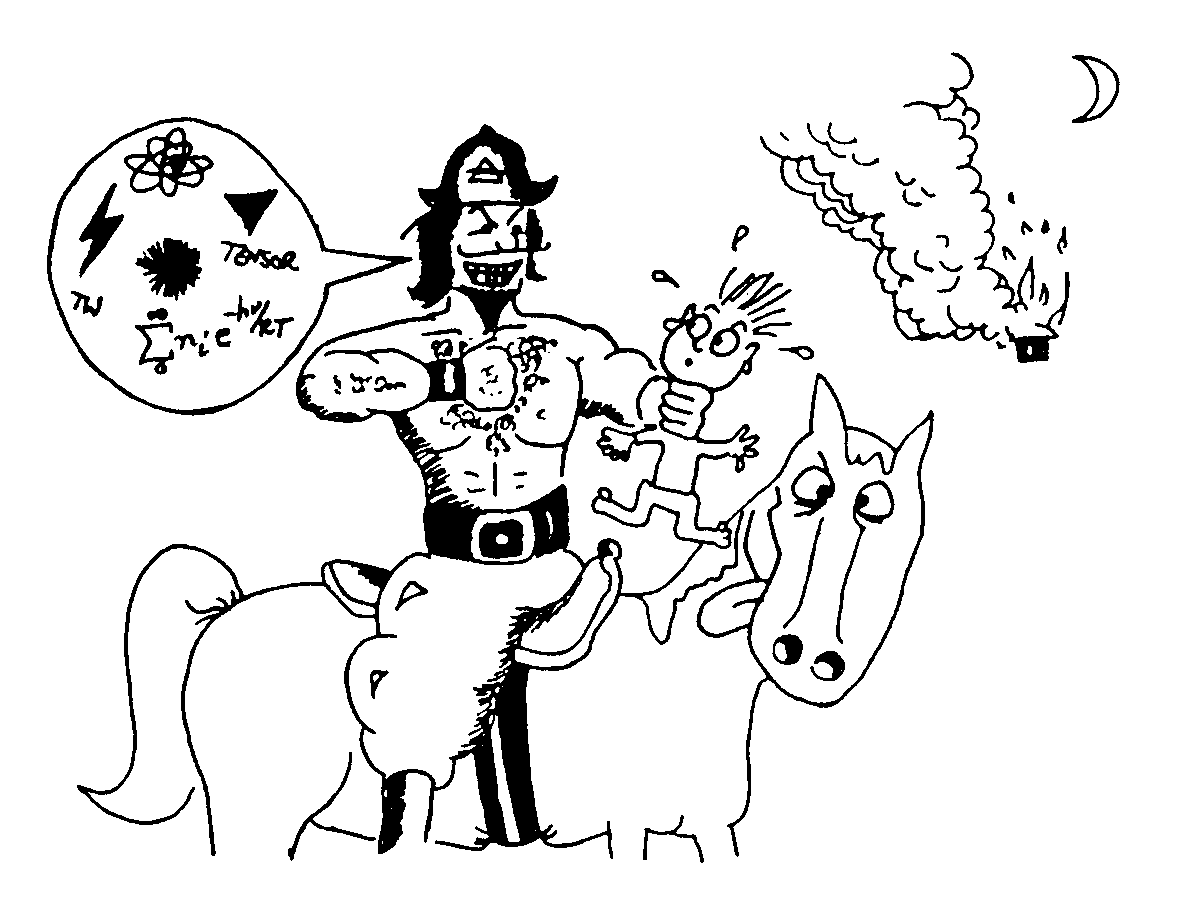
\includegraphics[width=\linewidth]{harjarv.png}
	\end{center}
	
	Ja, nu skall vi ut och härja,\\
	supa och slåss och svärja,\\
	bränna röda stugor,\\
	slå små barn och säga fula ord.\\
	Med blod skall vi stäppen färga.\\
	Nu, änteligen, lär ja'\\
	kunna dra nå'n verklig nytta\\
	av min Hermodskurs i mord!
	
    \showversenumber
	Hurra, nu skall man äntligen få röra på benen,\\
	hela stammen jublar och det spritter i grenen.\\
	Tänk att än en gång få rida fram\\
	på Brunte i galopp!\\
	Din doft, o kära Brunte, är trots brist i hygienen\\
	för en vild mongol minst lika ljuv som syrenen.\\
	Tänk att på din rygg få rida\\
	runt i sta'n och spela topp!
	
	Ja, nu skall vi ut \ldots{}
	
    \showversenumber
	Ja, mordbränder är klämmiga, tag fram fotogenen!\\
	Eftersläckningen tillhör just de fenomenen\\
	inom brandmansyrket, som jag\\
	tycker är nå'n nytta med.\\
	Jag målar för mitt inre upp den härliga scenen:\\
	blodrött mitt i brandgult. Ej ens prins Eugen en\\
	lika mustig vy kan måla\\
	ens om han målade med sked.
	
	Ja, nu skall vi ut \ldots{}
	
\end{song}
